\documentclass[tikz,border=8pt]{standalone}
% Shared look for every TikZ diagram. Load with \input{../../tools/tikz-style.tex}
\usepackage[sfdefault]{roboto}
\usetikzlibrary{arrows.meta, positioning, shapes.geometric, calc, fit, backgrounds}
\definecolor{cblue}{HTML}{4C78A8}
\definecolor{corange}{HTML}{F58518}
\definecolor{cgreen}{HTML}{54A24B}
\definecolor{cred}{HTML}{E45756}
\definecolor{cpurple}{HTML}{B279A2}
\definecolor{cgrey}{HTML}{6B6B6B}
\tikzset{
  every picture/.style={font=\sffamily, line width=1.2pt},
  box/.style={draw=#1, fill=#1!12, rounded corners=4pt, align=center, inner sep=7pt, minimum height=1.1cm},
  box/.default=cgrey,
  arrow/.style={-{Stealth[length=3mm]}, draw=cgrey, line width=1.4pt},
  title/.style={font=\sffamily\bfseries\Large},
  note/.style={font=\sffamily\small, text=cgrey, align=center},
}
\AtBeginDocument{\hyphenpenalty=10000 \exhyphenpenalty=10000}

% Explicit graph: all vertices and edges are built and stored before the search starts (fine for the room's 76 cells).
% Implicit graph: only the cells the search has reached are stored; a successor function returns a cell's free neighbours when the search
% asks, so only the cells the search touches are ever made (CMU 16-350 slides; CS188 1.2.2; Khemani lecture 8).
\begin{document}
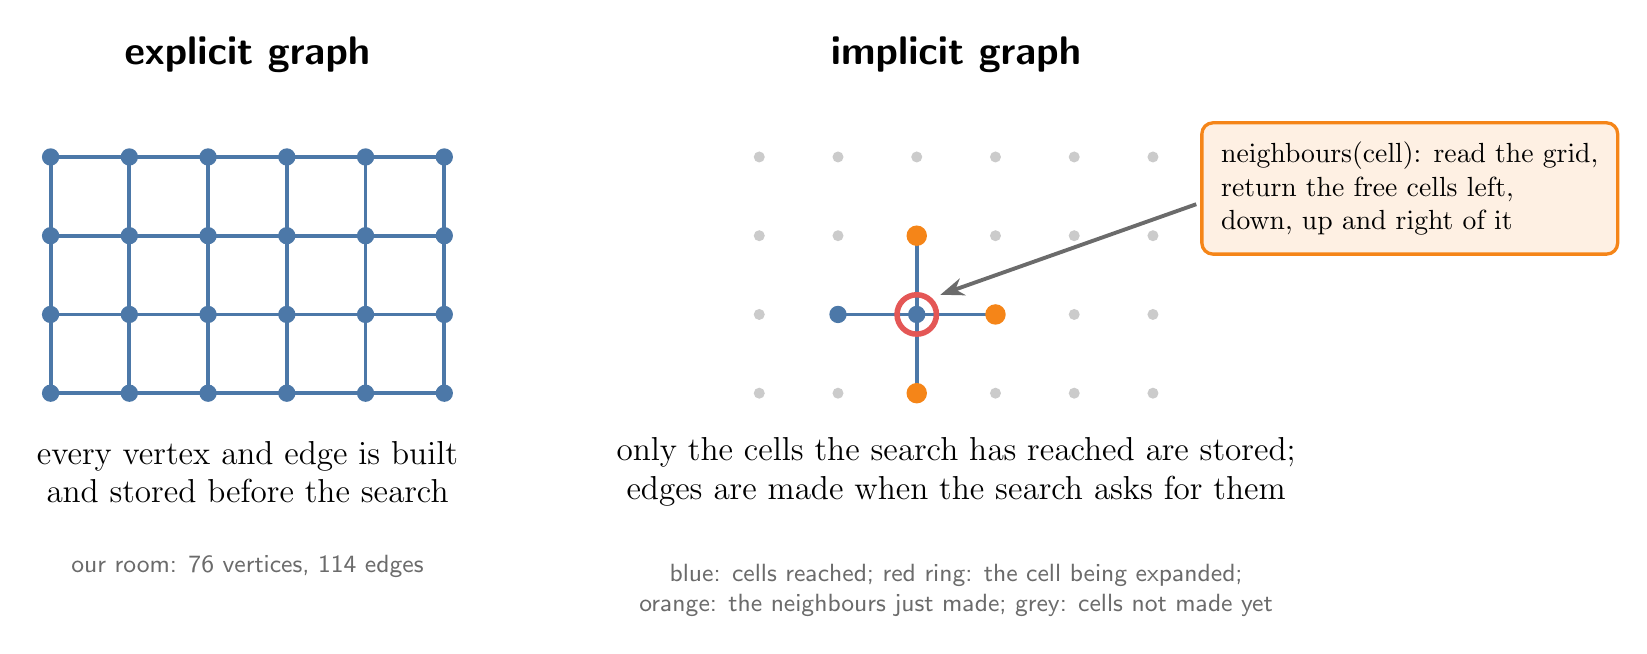
\begin{tikzpicture}[every node/.append style={font=\large}]
  % left: explicit
  \node[title] at (2.5,4.3) {explicit graph};
  \foreach \i in {0,...,5} \foreach \j in {0,...,3} {
    \ifnum\i<5 \draw[cblue, line width=1.4pt] (\i,\j) -- (\i+1,\j); \fi
    \ifnum\j<3 \draw[cblue, line width=1.4pt] (\i,\j) -- (\i,\j+1); \fi
  }
  \foreach \i in {0,...,5} \foreach \j in {0,...,3} \fill[cblue] (\i,\j) circle (0.11);
  \node[align=center] at (2.5,-1.0) {every vertex and edge is built\\and stored before the search};
  \node[note] at (2.5,-2.2) {our room: 76 vertices, 114 edges};
  % right: implicit
  \begin{scope}[xshift=9cm]
    \node[title] at (2.5,4.3) {implicit graph};
    \foreach \i in {0,...,5} \foreach \j in {0,...,3} \fill[cgrey!35] (\i,\j) circle (0.07);
    \draw[cblue, line width=1.4pt] (1,1) -- (2,1) (2,1) -- (2,2) (2,1) -- (3,1) (2,1) -- (2,0) (2,1) -- (1,1);
    \foreach \p in {(1,1),(2,1)} \fill[cblue] \p circle (0.11);
    \foreach \p in {(3,1),(2,2),(2,0)} \fill[corange] \p circle (0.13);
    \draw[cred, line width=2pt] (2,1) circle (0.25);
    \node[box=corange, anchor=west, font=\normalsize, align=left] at (5.6,2.6)
      {neighbours(cell): read the grid,\\return the free cells left,\\down, up and right of it};
    \draw[arrow] (5.55,2.4) -- (2.3,1.25);
    \node[align=center] at (2.5,-1.0) {only the cells the search has reached are stored;\\edges are made when the search asks for them};
    \node[note, align=center] at (2.5,-2.5) {blue: cells reached; red ring: the cell being expanded;\\orange: the neighbours just made; grey: cells not made yet};
  \end{scope}
\end{tikzpicture}
\end{document}
